\documentclass[12pt]{article}
\usepackage[english]{babel}
\usepackage{geometry}
\usepackage{amssymb}
\usepackage{acronym}
\usepackage{float}
\usepackage{graphicx}
\usepackage{listings}
\usepackage{color}
\usepackage{verbatim}
\usepackage{subcaption}
\usepackage{multicol}
\usepackage{wrapfig}
\usepackage[colorlinks,pdfpagelabels,pdfstartview = FitH,bookmarksopen = true,bookmarksnumbered = true, ,plainpages = false,hypertexnames = false, citecolor=blue,filecolor=blue,linkcolor=blue,urlcolor=blue] {hyperref}


\geometry{a4paper,left=1.5cm,right=1.5cm, top=1.5cm, bottom=1.5cm}


\setlength{\parindent}{0pt} % Kein Einzug
\begin{document}

%\listoffigures
%\listoftables
%\lstlistoflistings
\newpage
\pagestyle{plain}
\setcounter{page}{1}

\textbf{\Huge Escape the University}\\

\begin{multicols}{2}
	\textbf{Escape the University} is a 3D single-character stealth-game.
	You play as a student who failed his exam completely and has to steal the evidence that the exam has happend, in order to be not graded with the help of an excuse. \\ \\
		Manuel Schrempf (e0920136)\\
		Stefan Wilker   (e0920293)

		\section*{Features}
		\begin{itemize}
			\item Singlecharacter
			\item First and third person
			\item Stealth elements
			\item Animated characters
			\item Explore university building
			\item Easter eggs
			\item Toggle light
			\item Shadows
			\item On screen text with self calculated \textit{signed distance fields}
		\end{itemize}
		\columnbreak

		\begin{figure}[H]
		
\includegraphics[width=1\columnwidth]{Images/poster.jpg}
	\end{figure}
\end{multicols}

\section*{Gameplay}

The character is controlling a figure in a first or third person view.
You can interact with different objects and walk freely through the different floors of the 3D building, but other NPCs, for example students, tutors, professors, assistants, staff members, facility managers etc. should not see you sneaking around, since this results into your ex-matriculation or simply game over.
The line of sight from NPCs is:

\begin{itemize}
	\item reduced by two thirds, if the character is ducked and in the darkness.
	\item reduced by one third, if the character is ducked or in the darkness.
	\item normal if the character is in the light.
\end{itemize}

If the character is behind an opague object he is also out of sight.
Sometimes the character can stand behind objects, sometimes the character will have to duck to stay out of sight.

\section*{Background story}
You control a student in a fictional university building who does have taken this studies seriously.
This is bad, he is bad, and he should feel bad, because the third try on the hardest exam is faild.
Why?
Not even the first question on the received exam makes any sense:

\begin{quote}
\textit{Elisa studies tibetic overtone singing in her tenth bachelor semester. She lays slightly drunk in the sun in the Arctic without sun oil and has nothing but the radio on. Calculate the orbit of Uranus's moon Oberon and derive the weather of the 22.12.1913 in Washington D.C and Woodrow Wilson's location at 7 P.M.}
\end{quote}

This and each other question read raises your stress level to a never known climax - you know you will fail your studies if you stay even one more minute.
The professor is still handing out the exam sheets, so you take a chance and somehow you manage to slip out of the room without being noticed, fortunately with the exam sheet in your hands.
On the most quiet place, the toilet room, you find yourself getting a clear mind with the cold water from the faucet.
Your silent and undetected escape of the university must succeed in order to head home and get a medical certificate from your father's friend to be able to \textit{prove} that on this very day you were not even near the university.
You should just have prepared better for this exam, but with the exam questions in your hands, there is a shimmer of hope to pass next time.
All evidence of your participation in the exam has to be ereased.

\section*{Controls}
You are able to control the main character with the keys W,A,S,D and arrow keys and to freely move and look around in the first or third person view.
Therefore, looking around corners without being noticed by NPCs is possible for you. By using the left or right click of the mouse you are able to interact with objects like doors or light switches.

\begin{table}[h!]
  \centering
  \label{table1}
  \begin{tabular}{p{2cm} | l l}
		\textbf{Key} & \textbf{Function}\\ \hline
		W & Walk forwards	\\
		A & Strafe left \\
		S & Walk backwards \\
		D & Strafe right \\

		Mouse & Look around\\
		Right click & interaction\\
		Left click & interaction\\

		 ESC & Quit game \\
		 F1 & Help \\
		 F2 & Show FPS \\
		 F3 & Wireframe mode on or off \\
		 F4 & Textur-Sampling-Quality: Nearest Neighbor/Bilinear\\
		 F5 & Mip Mapping-Quality: Off/Nearest Neighbor/Linear\\
		 F6 & Depth visualization on or off\\
		 F7 & Pause or Resume game \\
		 F8 & Viewfrustum-Culling on/off\\
		 F9 & Blending on/off\\
  \end{tabular}
\end{table}


\section*{Technical Details}
\subsection*{Types of objects in the Game}

All objects in the scene are textured and illuminated. The following distinct object types are rendered:
\begin{itemize}
	\item NPCs
	\item Walls, pictures and graffitty on the walls, but only few
	\item Plants
	\item Rooms, name tags / signs on doors, conspiracy wirtings on the toiled
	\item Furnitures, books, bookshelfs, pc, monitors, bakets, lecture hall, black board, projector, overhead projector, chairs
	\item Interactable objects
	\item Windows
	\item Laterns
\end{itemize}

\subsection*{Camera}
A typical third person camera behind the played character controlled by the mouse to swing up, down, left and right which automatically follow the character from a distance of several meters.

\subsection*{Illumination}
The university is a normal illuminated building with switches to turn the light off and on. This means nearly every room, corridor, or courtyard is lit by a light blub or floodlight. Haruki Murakami once said:

\begin{quote}
\textit{Where there is light, there must be shadow, where there is shadow there must be light. There is no shadow without light and no light without shadow. [...]}
\end{quote}

So light and shadow will be implemented as stated in the effect list.

\subsection*{Collision Detection}
For being able to determine whether the line of sight of a NPC is crossed or not collision detection is needed. Of course if you ran into a NPC you will be detected too.

\subsection*{Effects}
The single effect lists may change according to the knowledge gained in the lecture, tutorial class, and through programming itself.

\begin{table}[h]
	\centering
	\begin{tabular}{l| l | p{11cm}}
		\textbf{Effect} & \textbf{Points} & \textbf{Description}\\
		\hline
		Deferred Shading & 1 & Use the Deferred Shading technique to speed up lighting for many light sources.
		It uses several render targets and processes light information (shadows etc) in a post process effect (decoupling it from the scenes geometry).
		Transparency, however, is more difficult to handle	\\
		\hline
		GPU Vertex Skinning &	2 &	A complete bone structure is loaded from a model file and assigned to the model according to weighted indices.
		The skinning is done on the GPU. \\
		\hline
		Shadow Maps (with PCF) & 1.5 & As presented in the lectures, shadow maps calculate the shadows via rendering the scene from the light source.
		PCF samples the shadow map several times to improve quality.
		Make sure to counter all artifacts.\\
	\end{tabular}
\end{table}


\section*{Sketches}
\begin{figure}[H]
	\center
		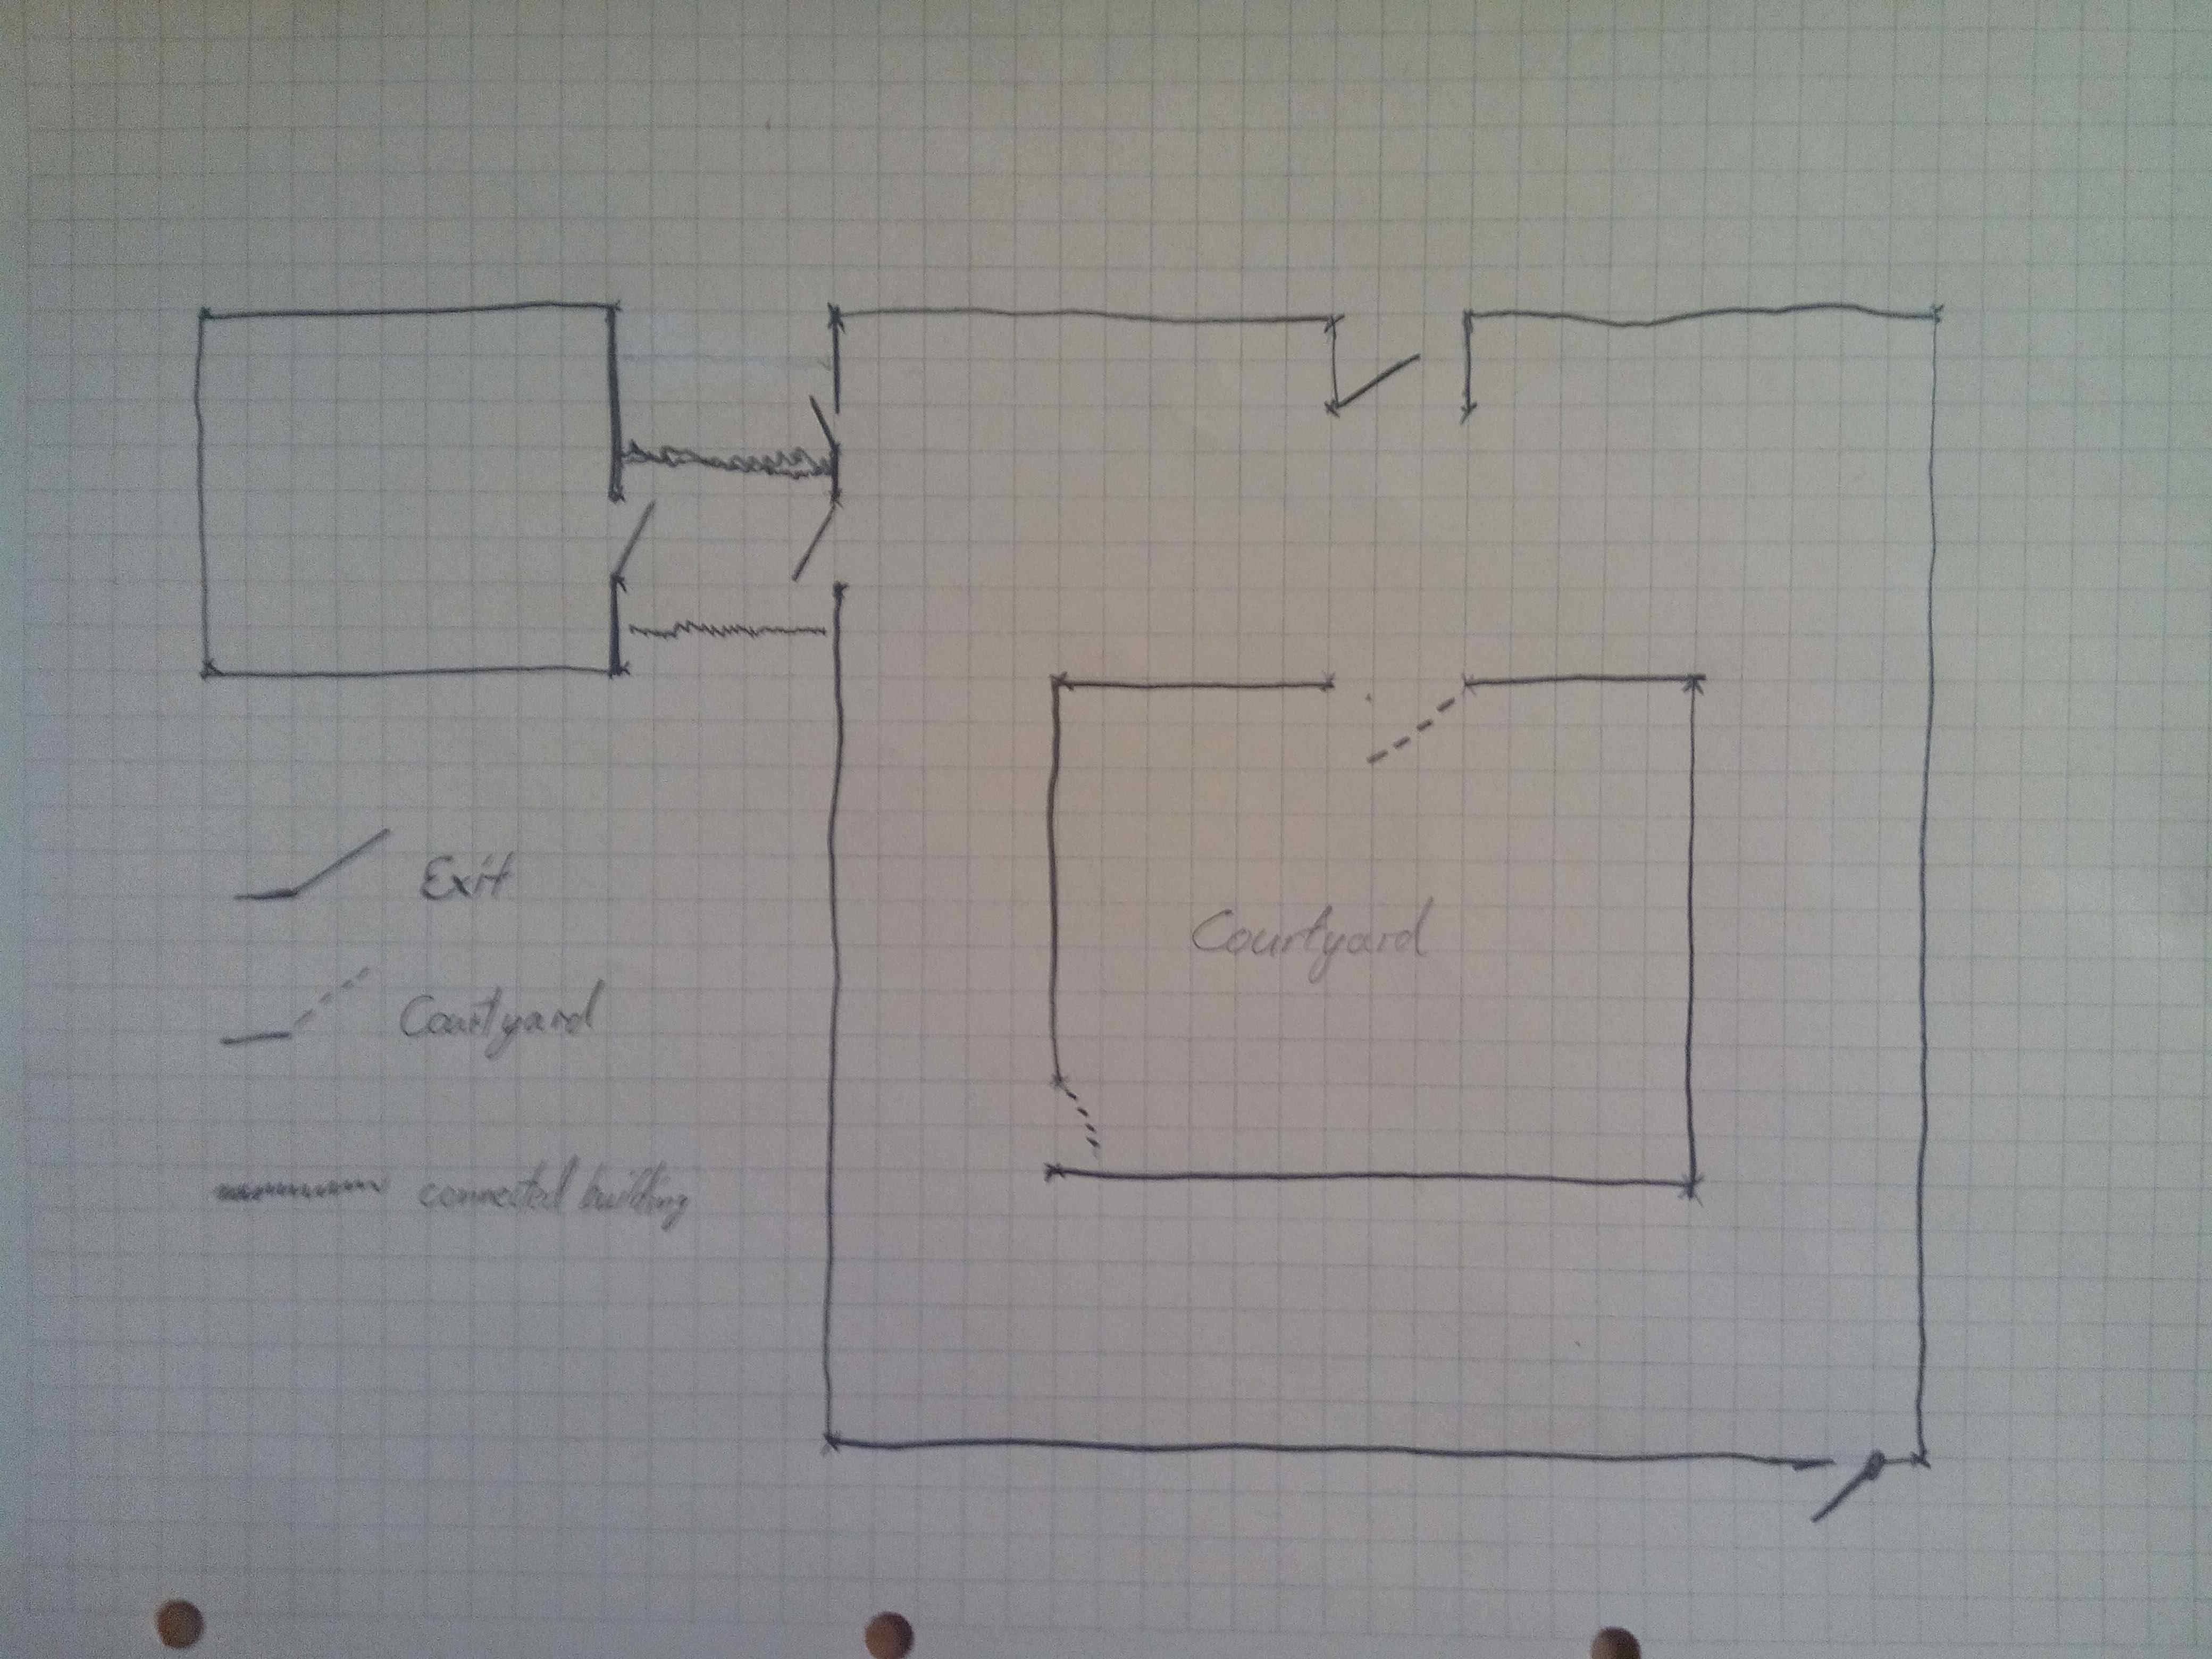
\includegraphics[width=0.9\textwidth]{Images/mapoverview}
		\caption{A first design on the first complex. You have to figure out, at which door you can Escape the University without being seen!}
\end{figure}
\begin{figure}
	\centering
	\begin{minipage}{0.45\textwidth}
		\centering
		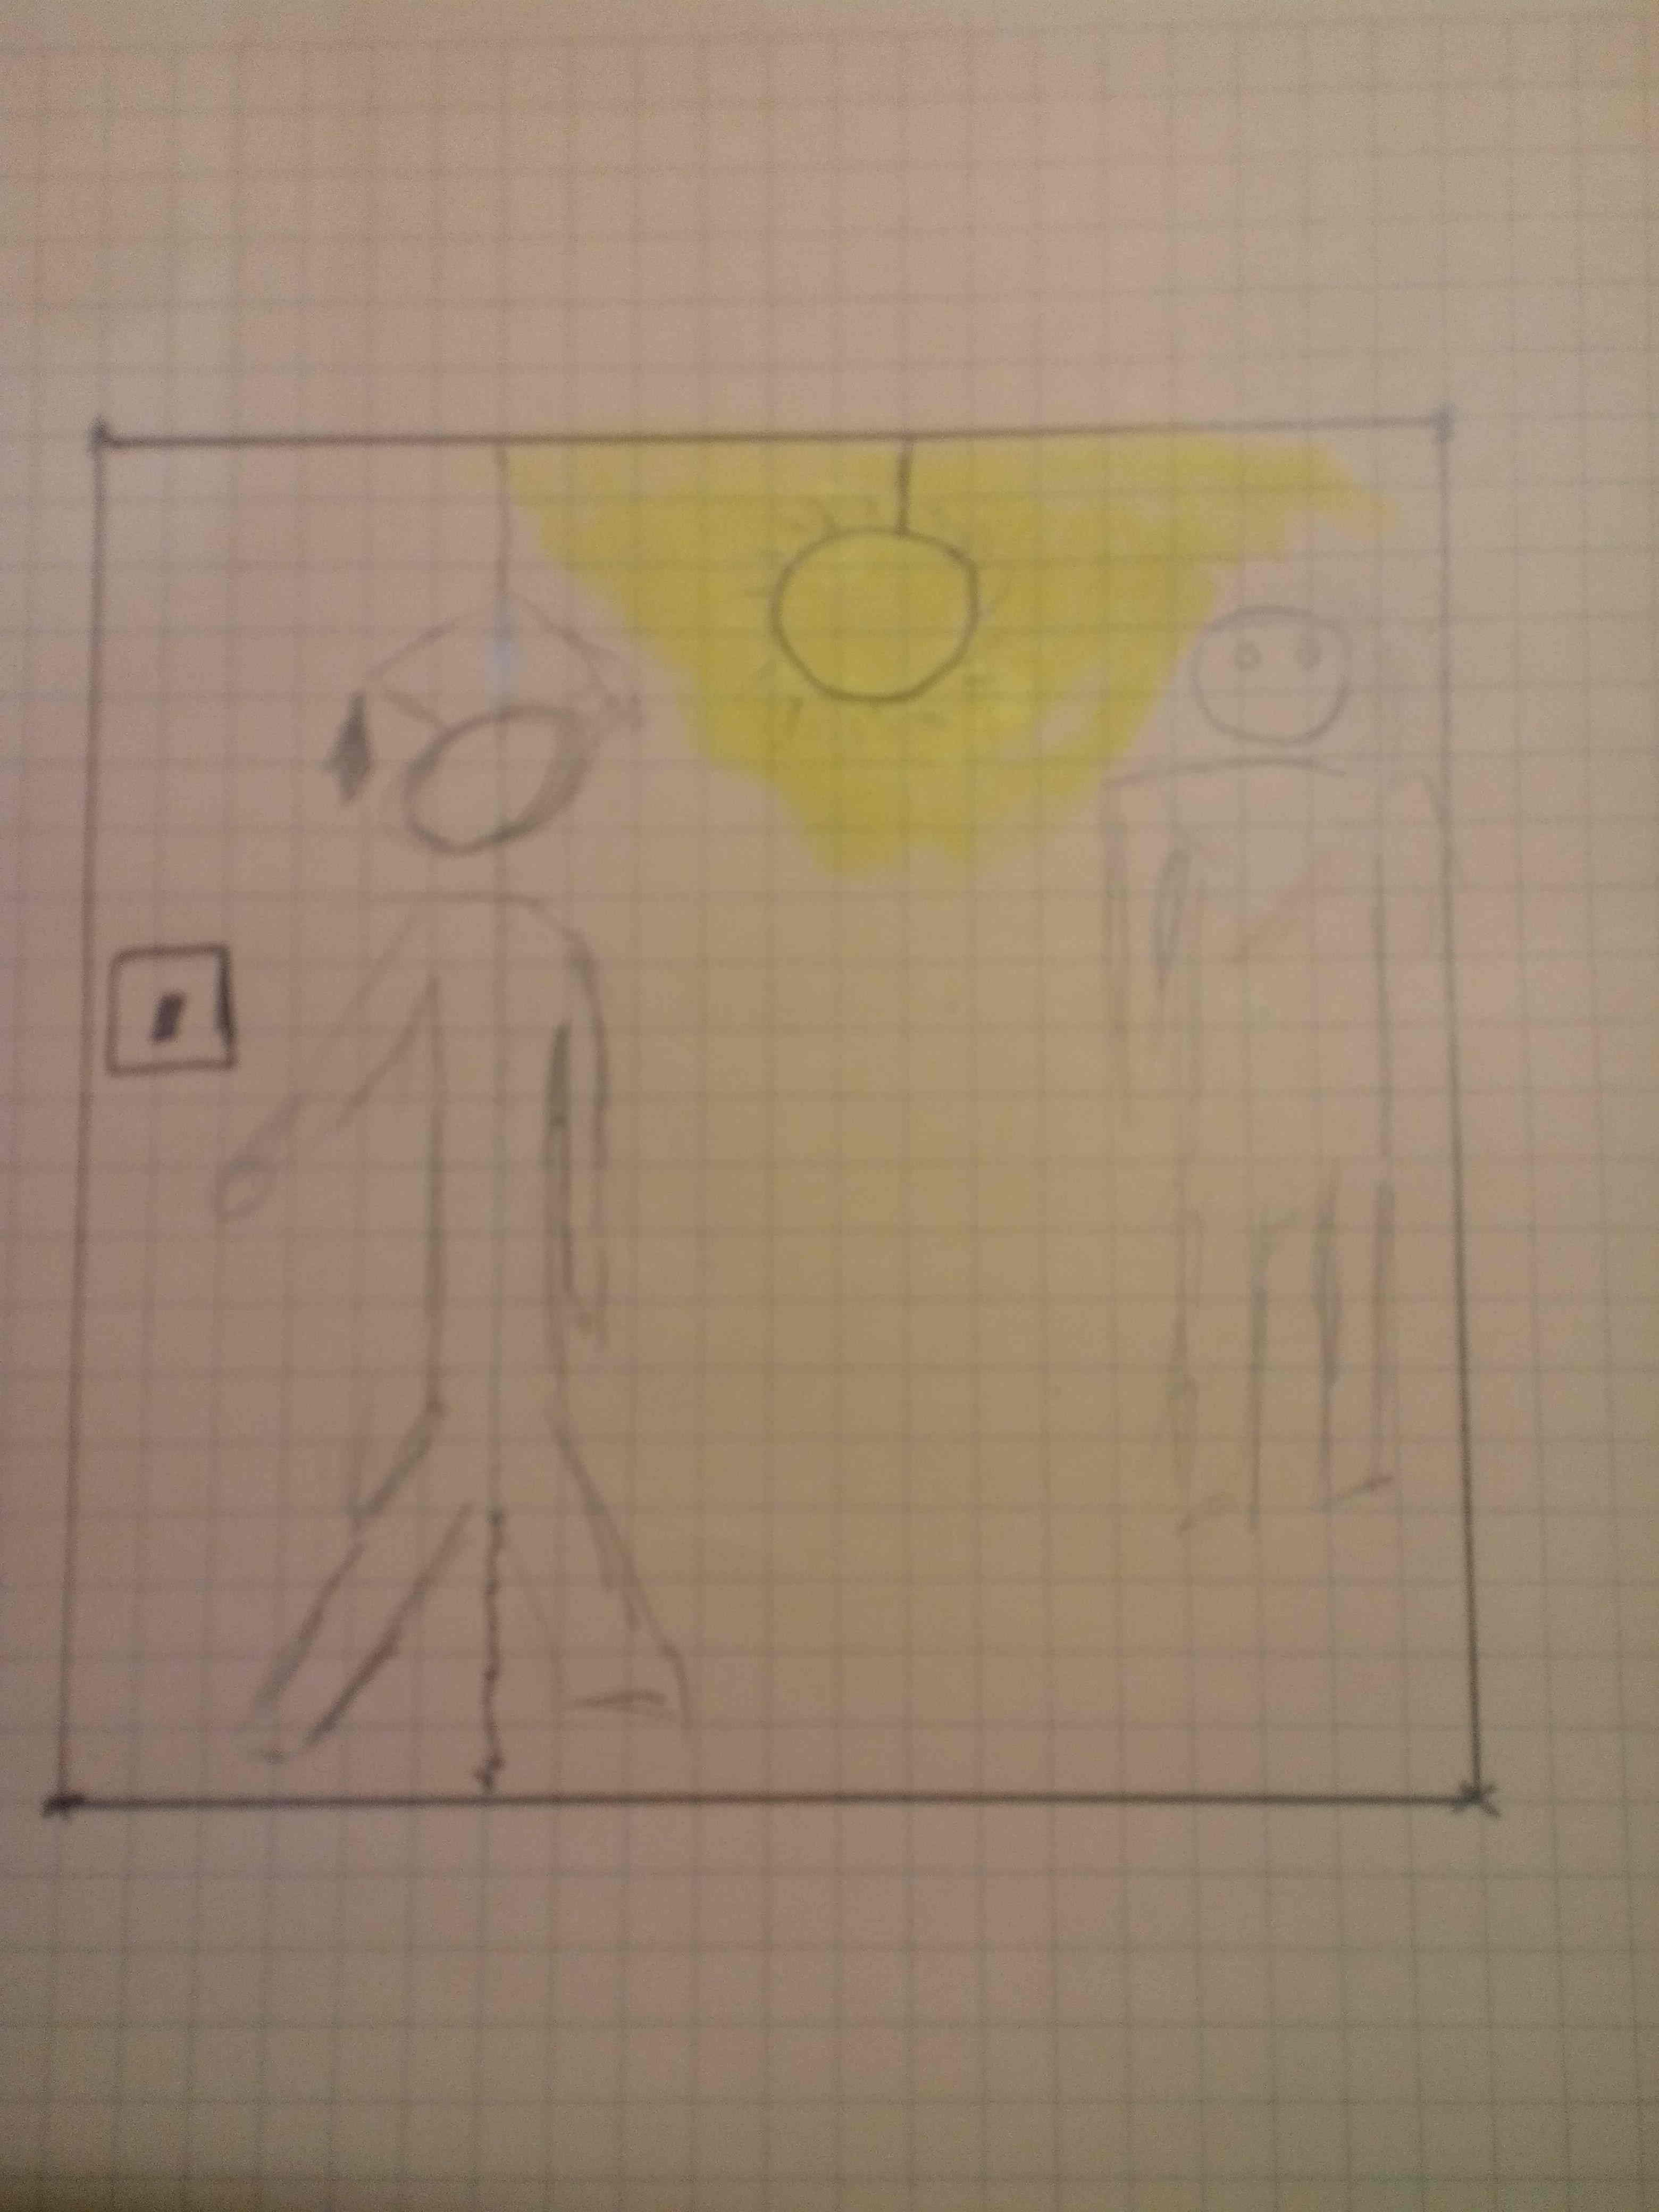
\includegraphics[width=0.9\textwidth]{Images/lighton} % first figure itself
		\caption{A sketch on the main character and an enemy. You must not move into his line of sight!}
	\end{minipage}\hfill
	\begin{minipage}{0.45\textwidth}
		\centering
		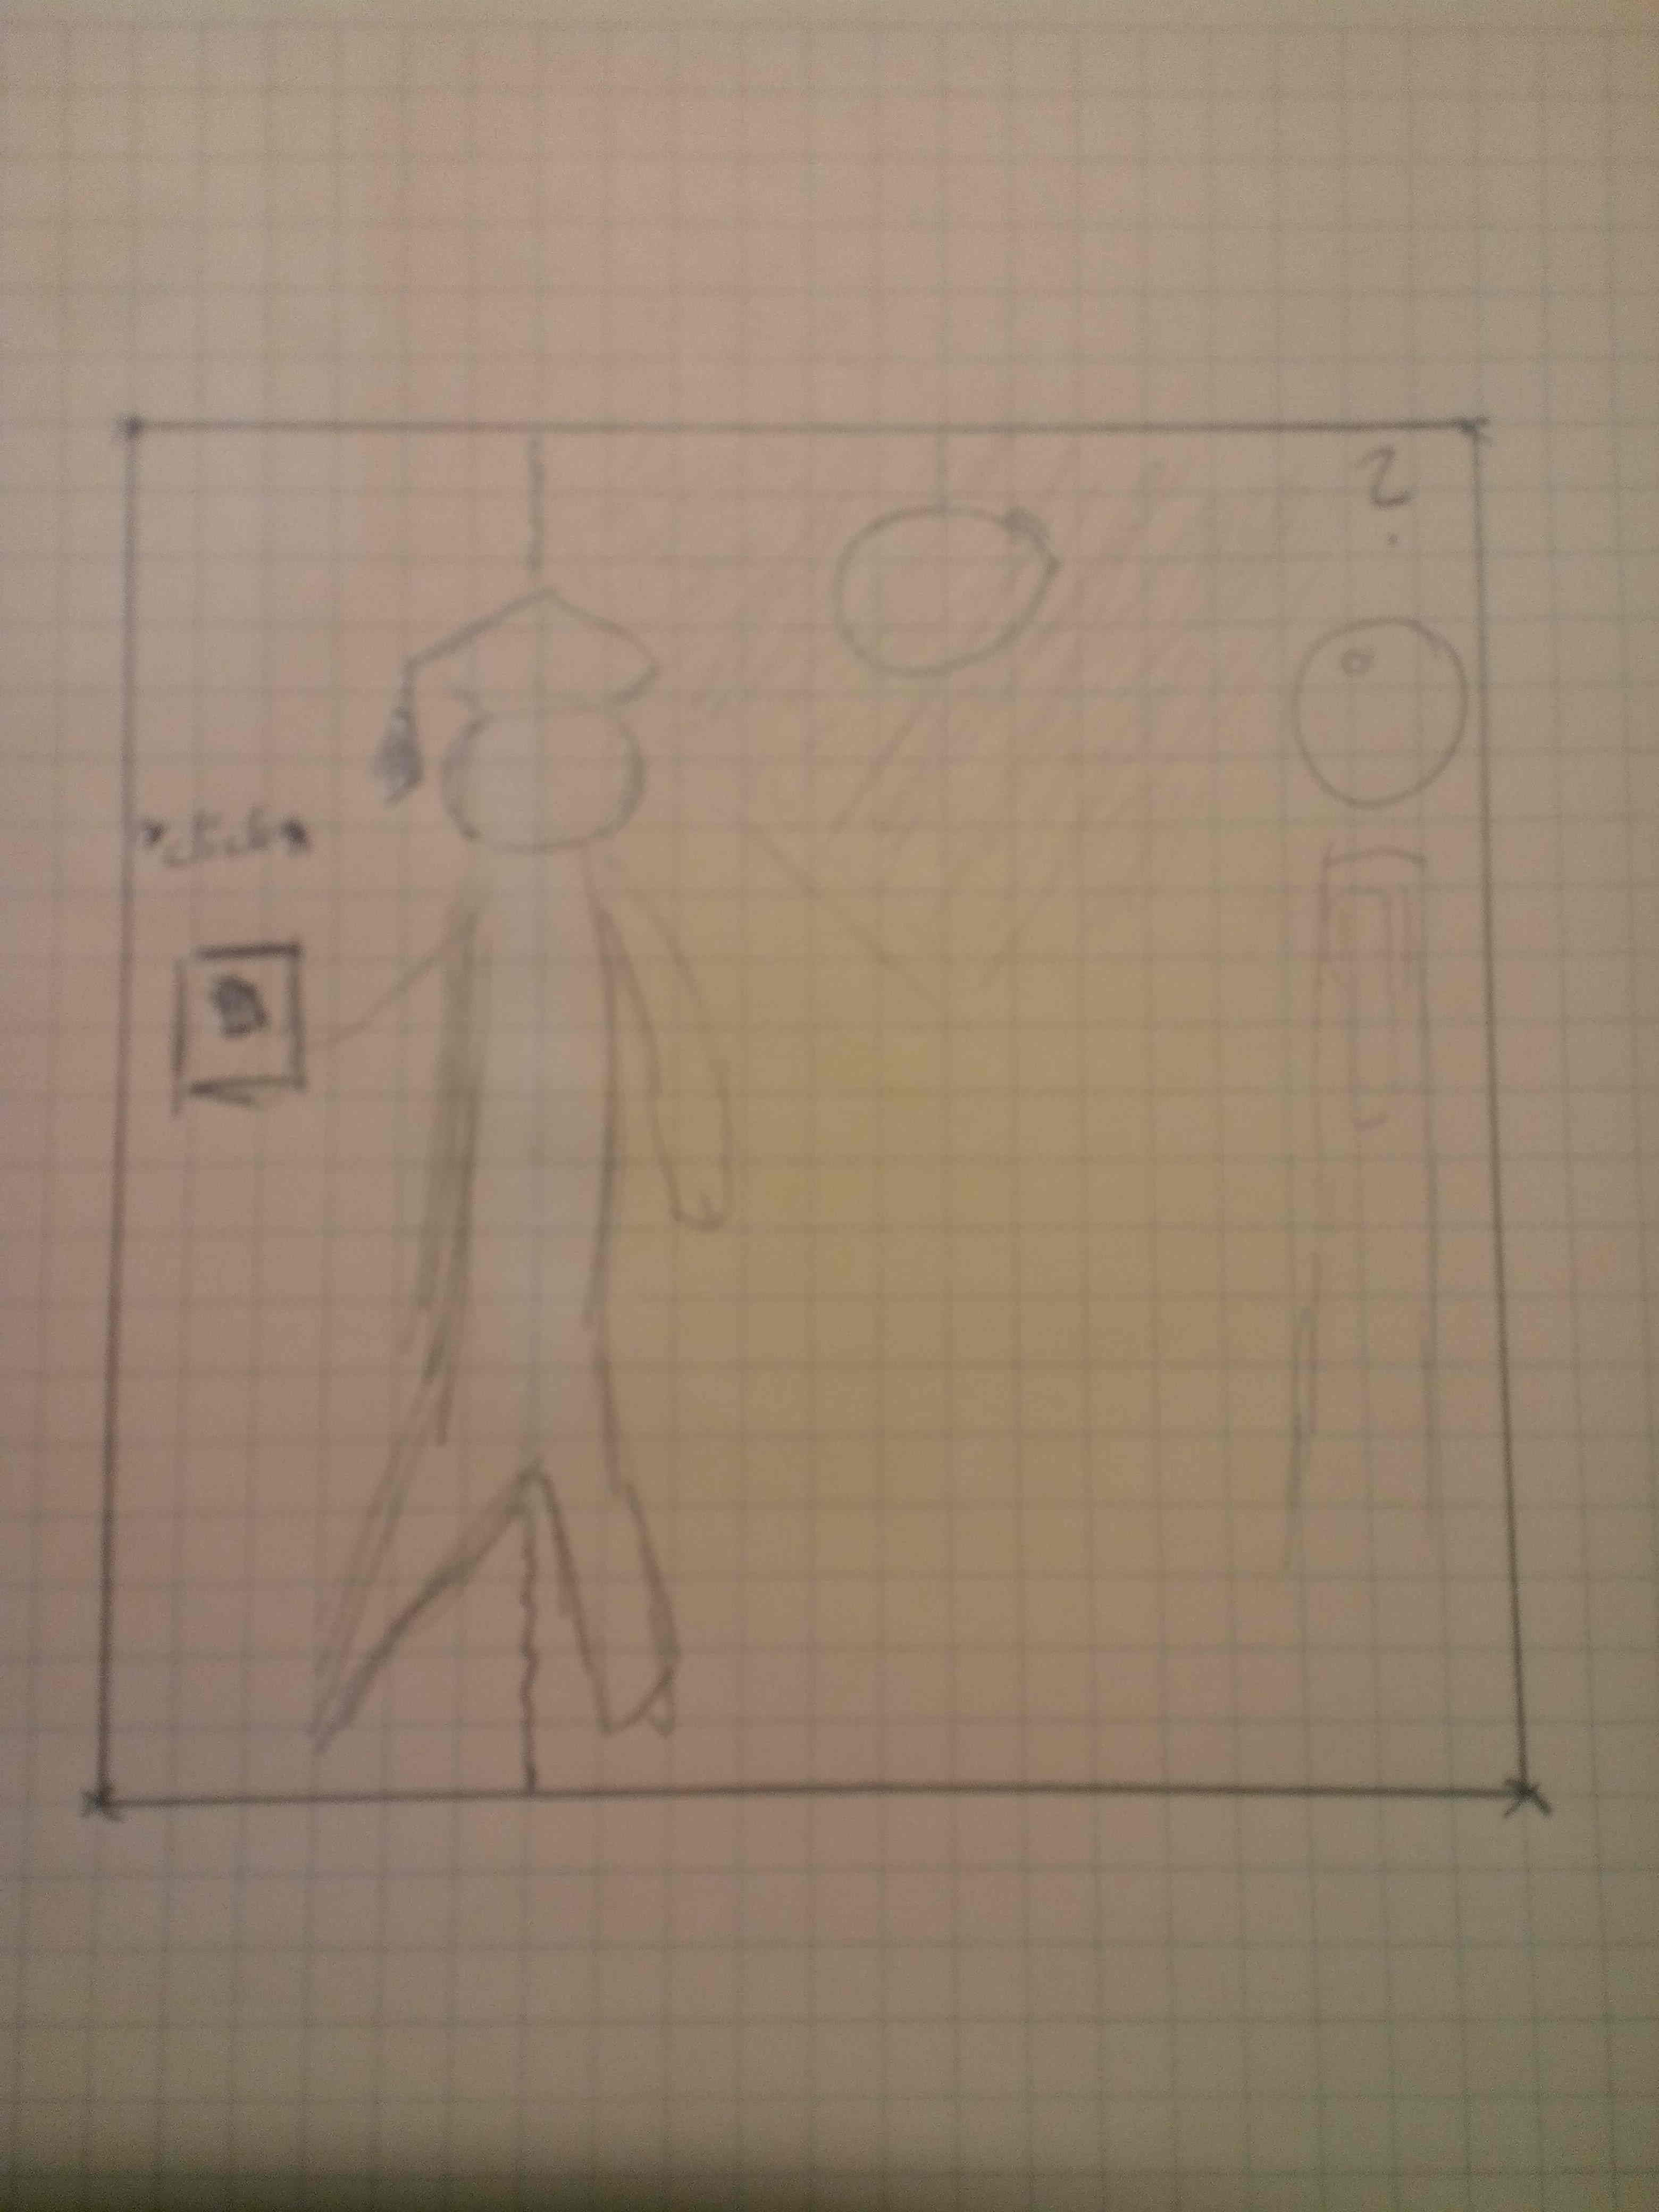
\includegraphics[width=0.9\textwidth]{Images/lightoff} % second figure itself
		\caption{After activating the switch, it is save to pass by.}
	\end{minipage}
\end{figure}
\begin{figure}
	\centering
	\begin{minipage}{0.45\textwidth}
		\centering
		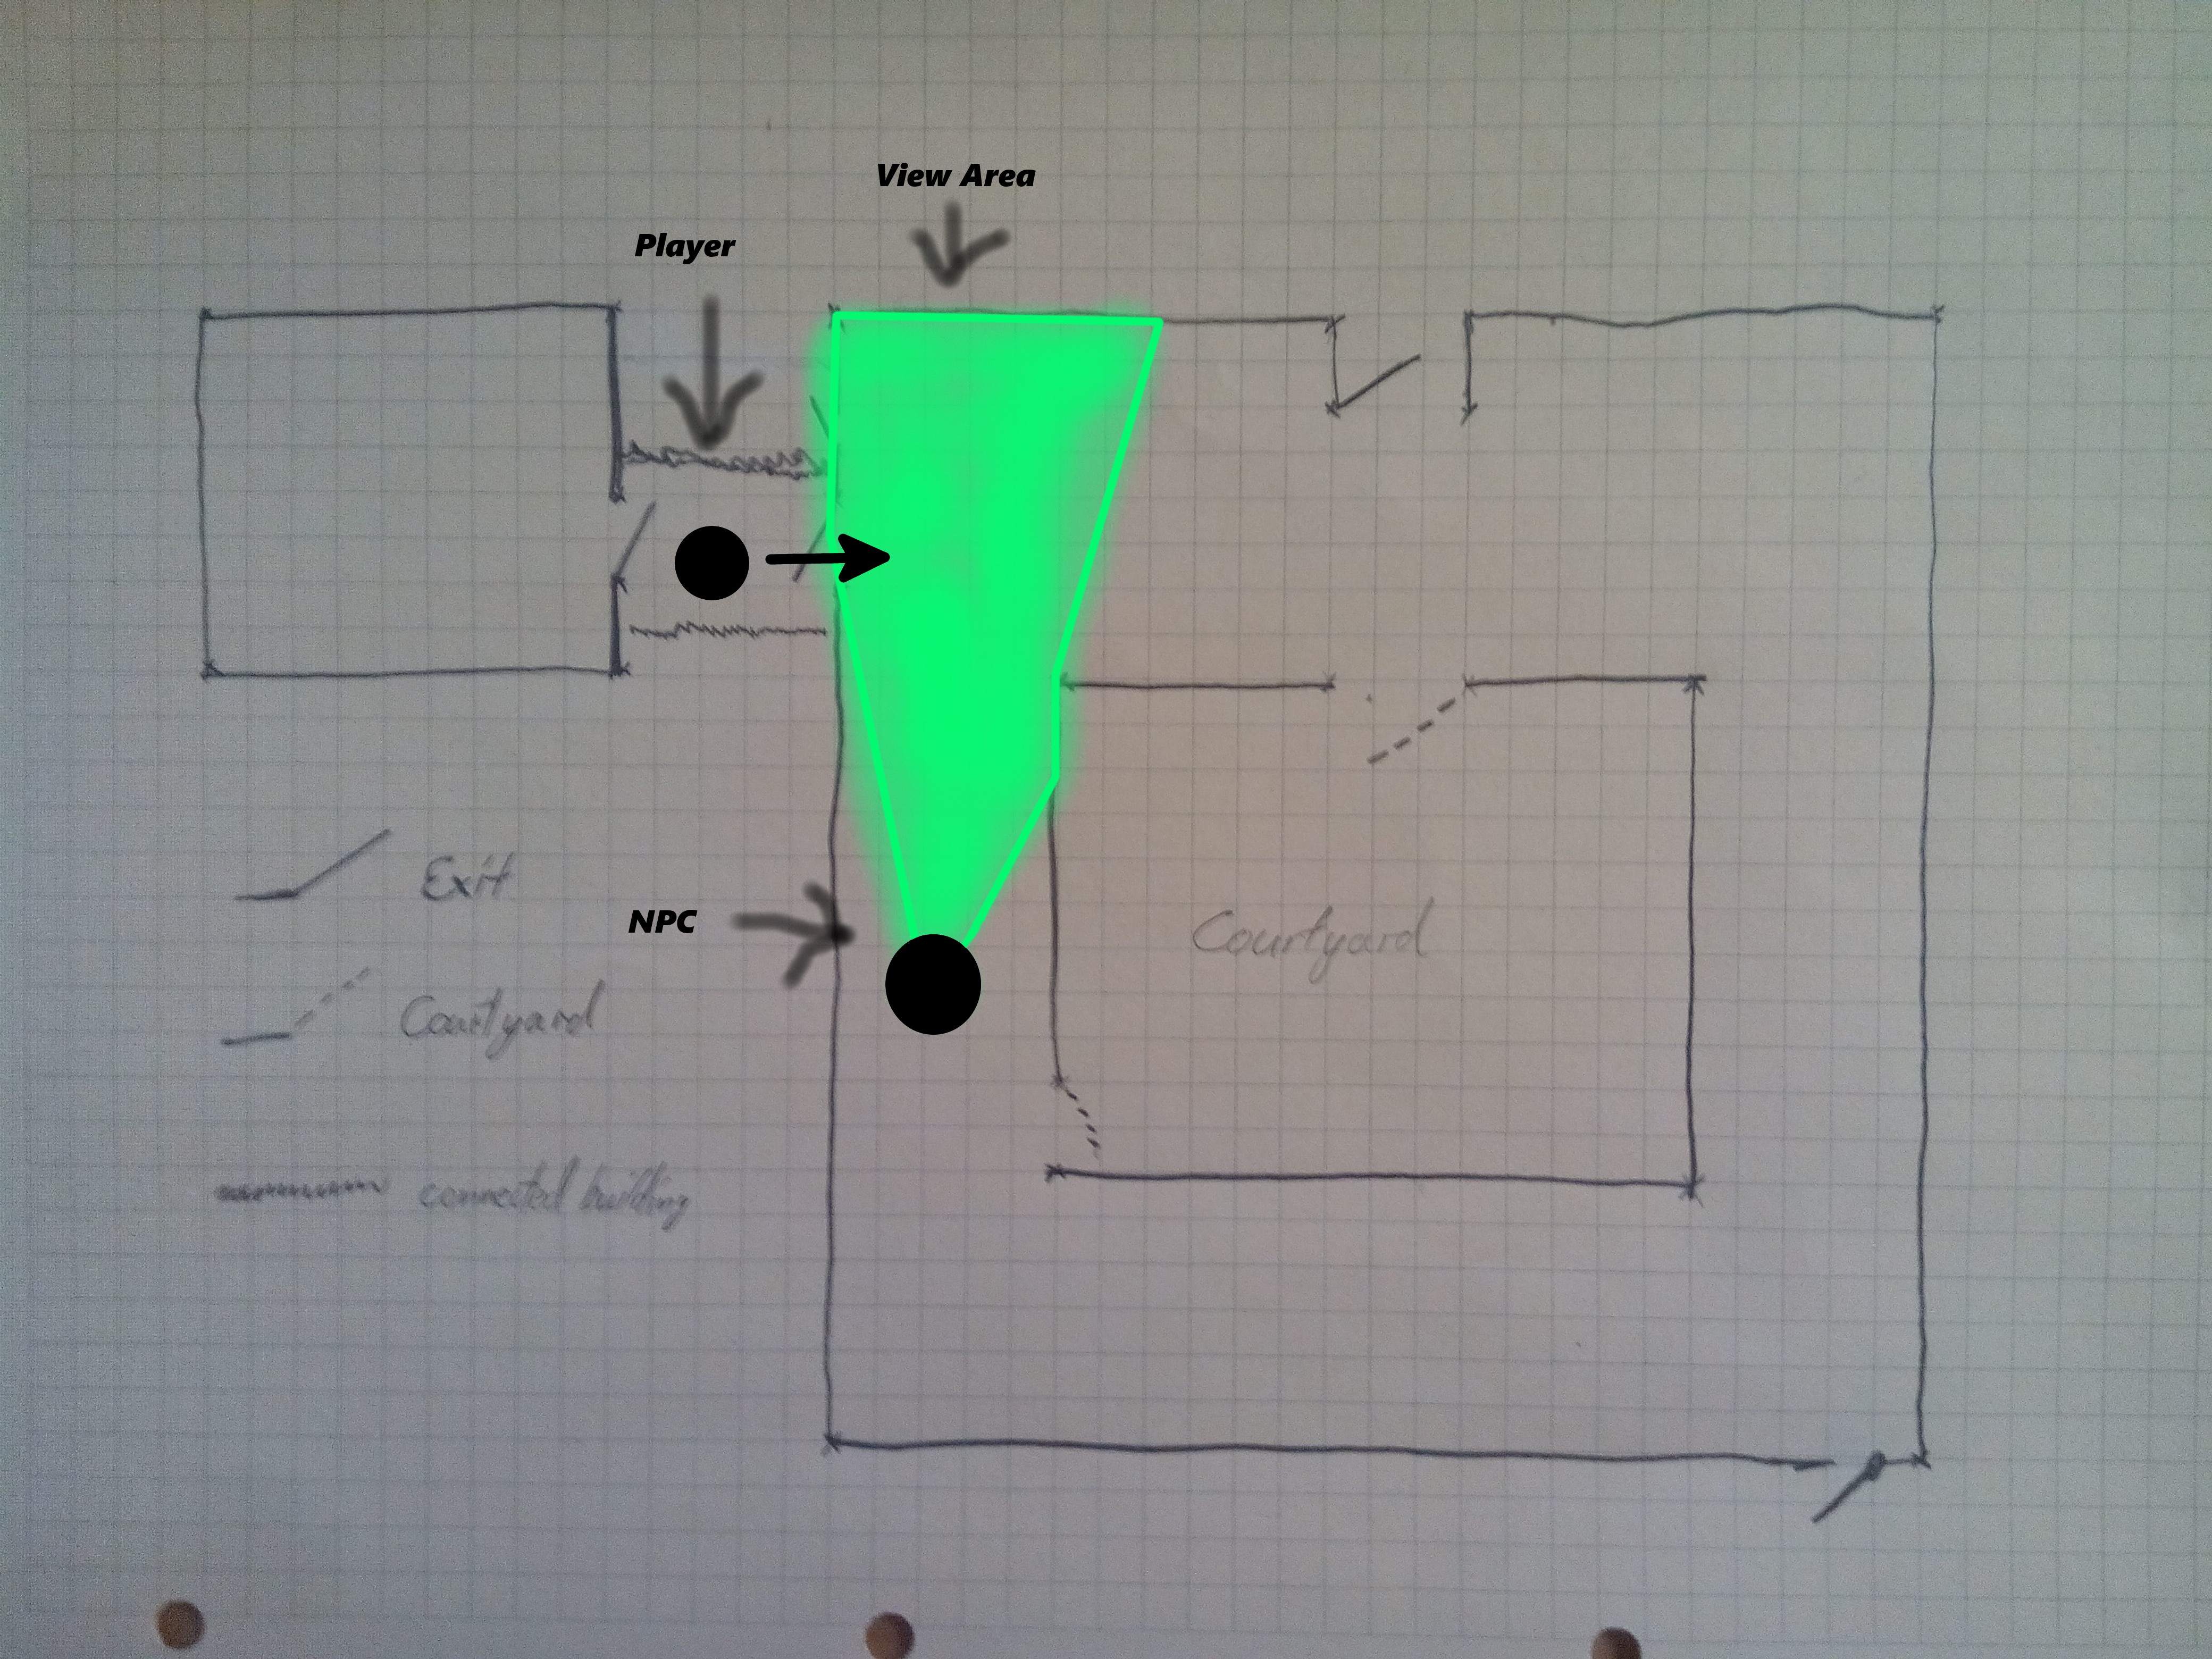
\includegraphics[width=0.9\textwidth]{Images/movingintosightfield} % first figure itself
		\caption{Moving forward...}
	\end{minipage}\hfill
	\begin{minipage}{0.45\textwidth}
		\centering
		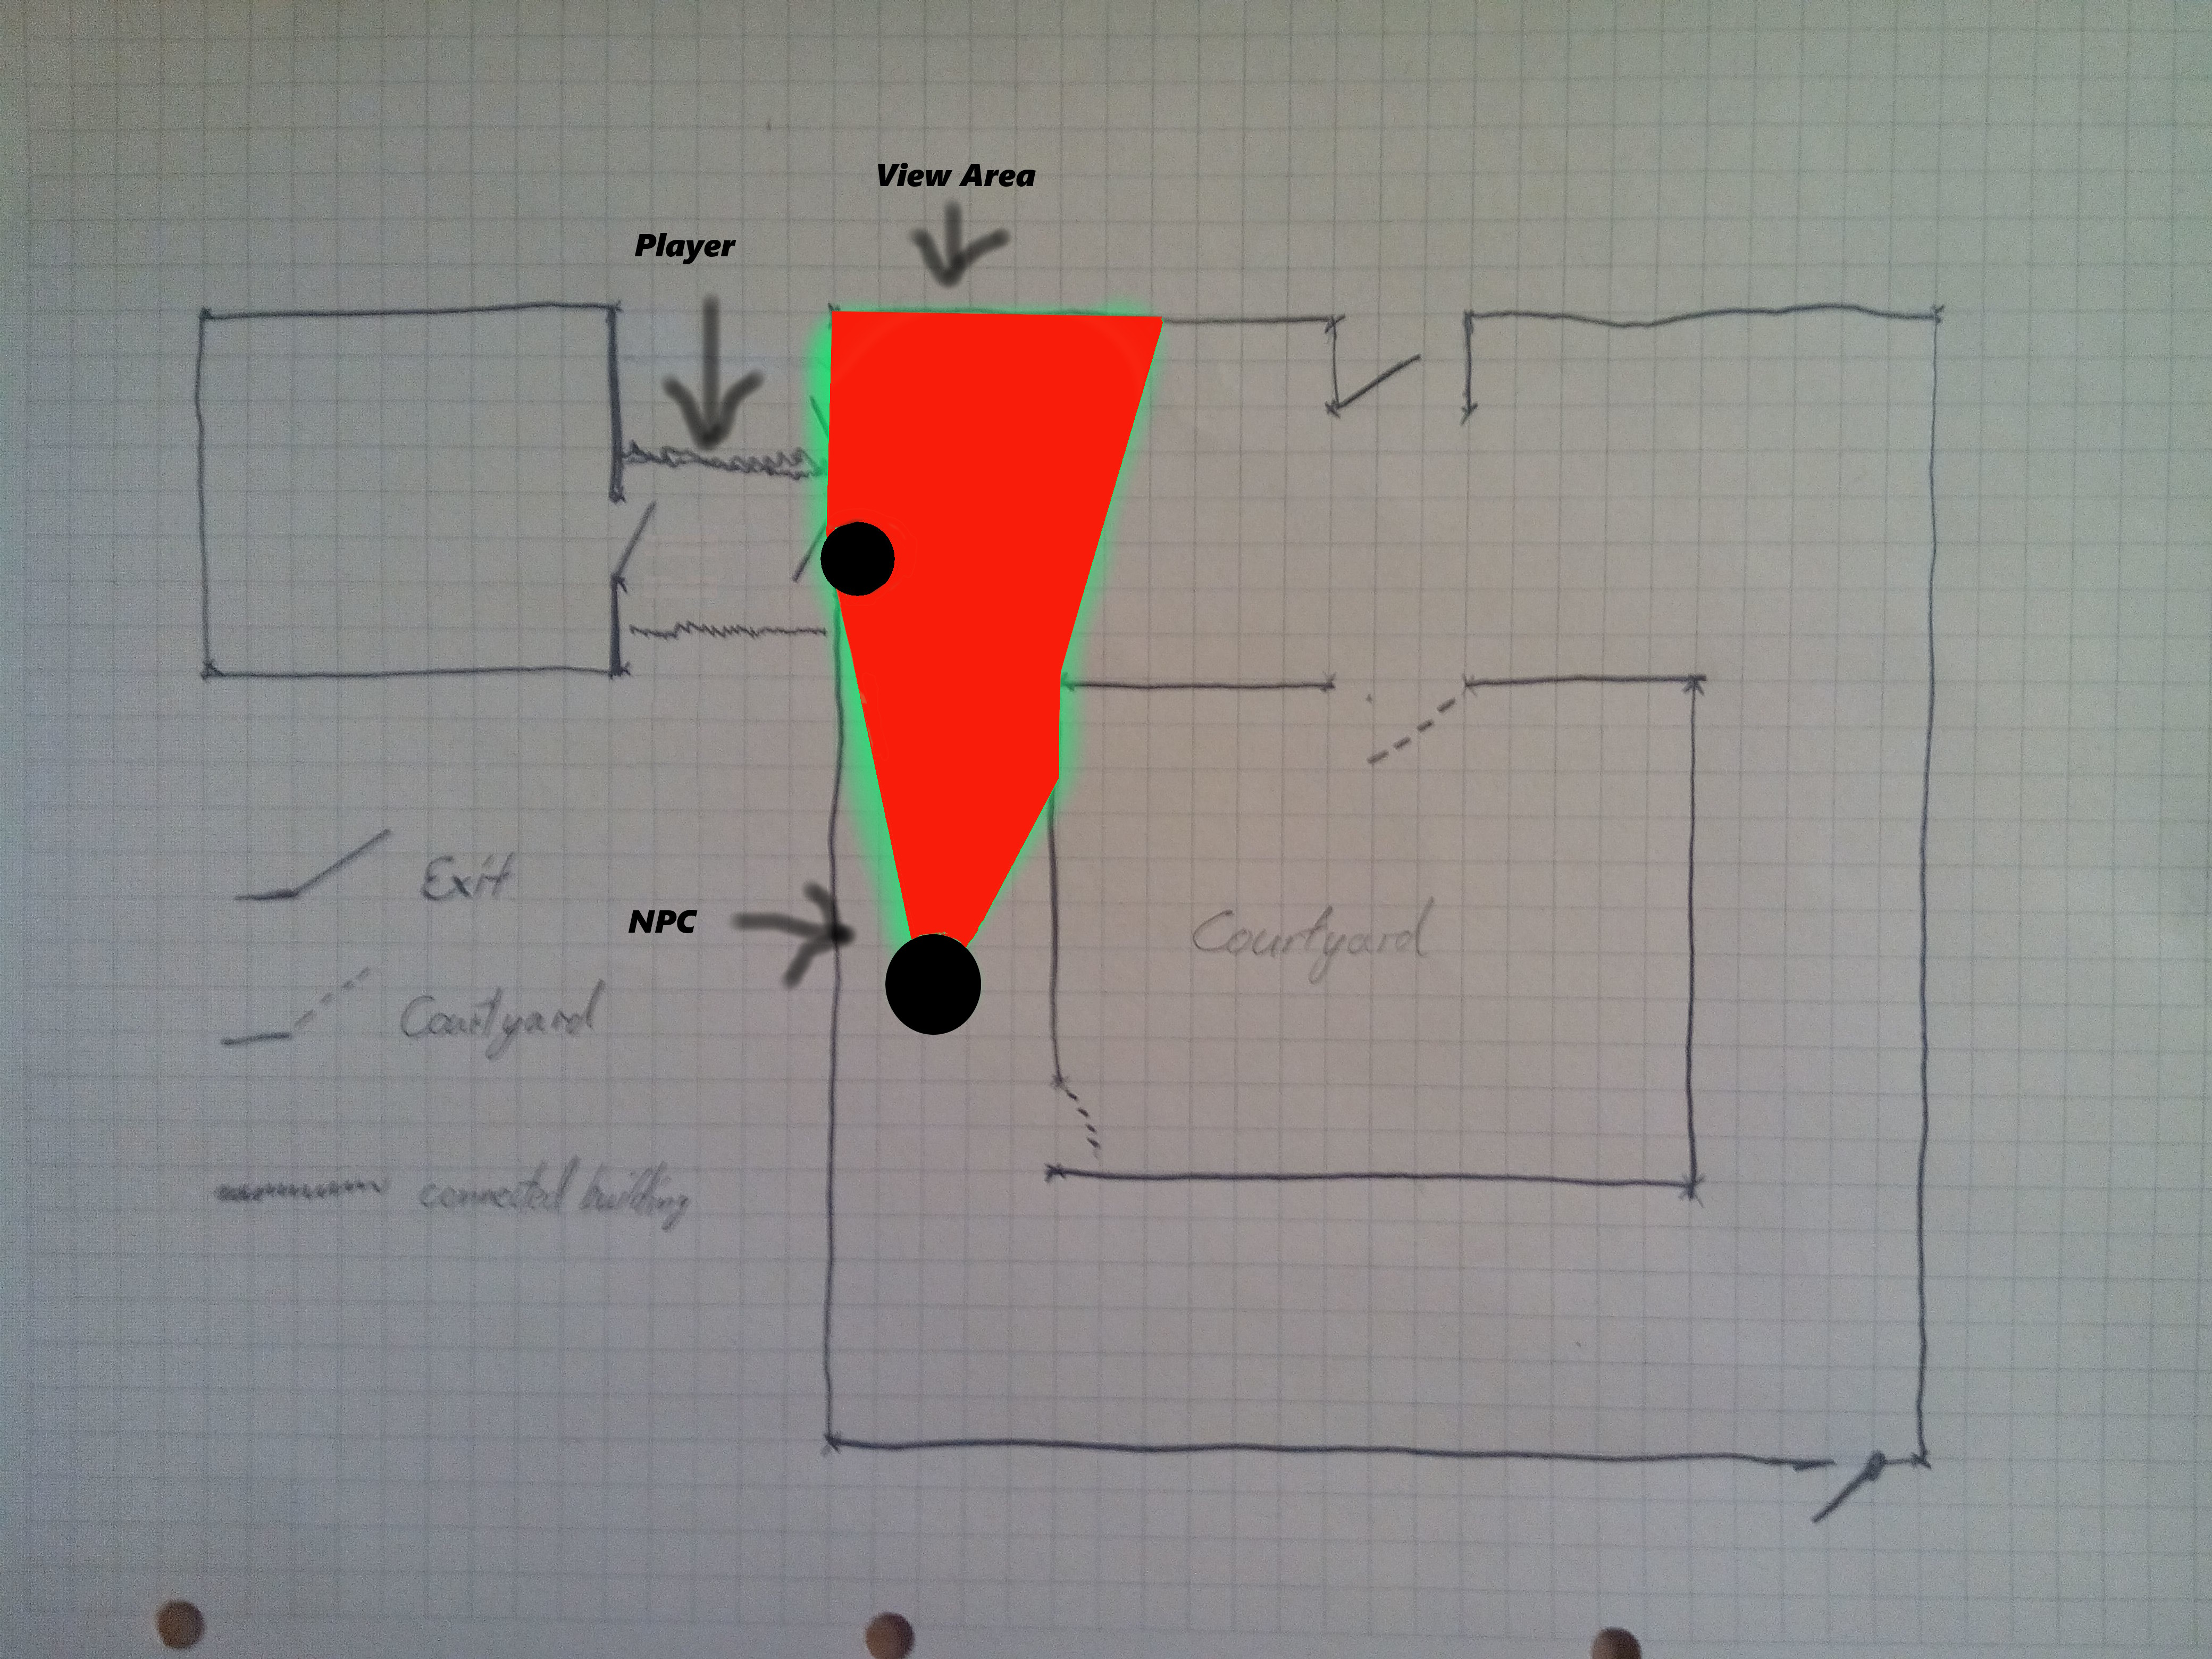
\includegraphics[width=0.9\textwidth]{Images/gotcaught} % second figure itself
		\caption{You ran into the line of sight... Game over man!}
	\end{minipage}
\end{figure}
 \begin{figure}
       	\centering
       	\begin{minipage}{0.45\textwidth}
       		\centering
       		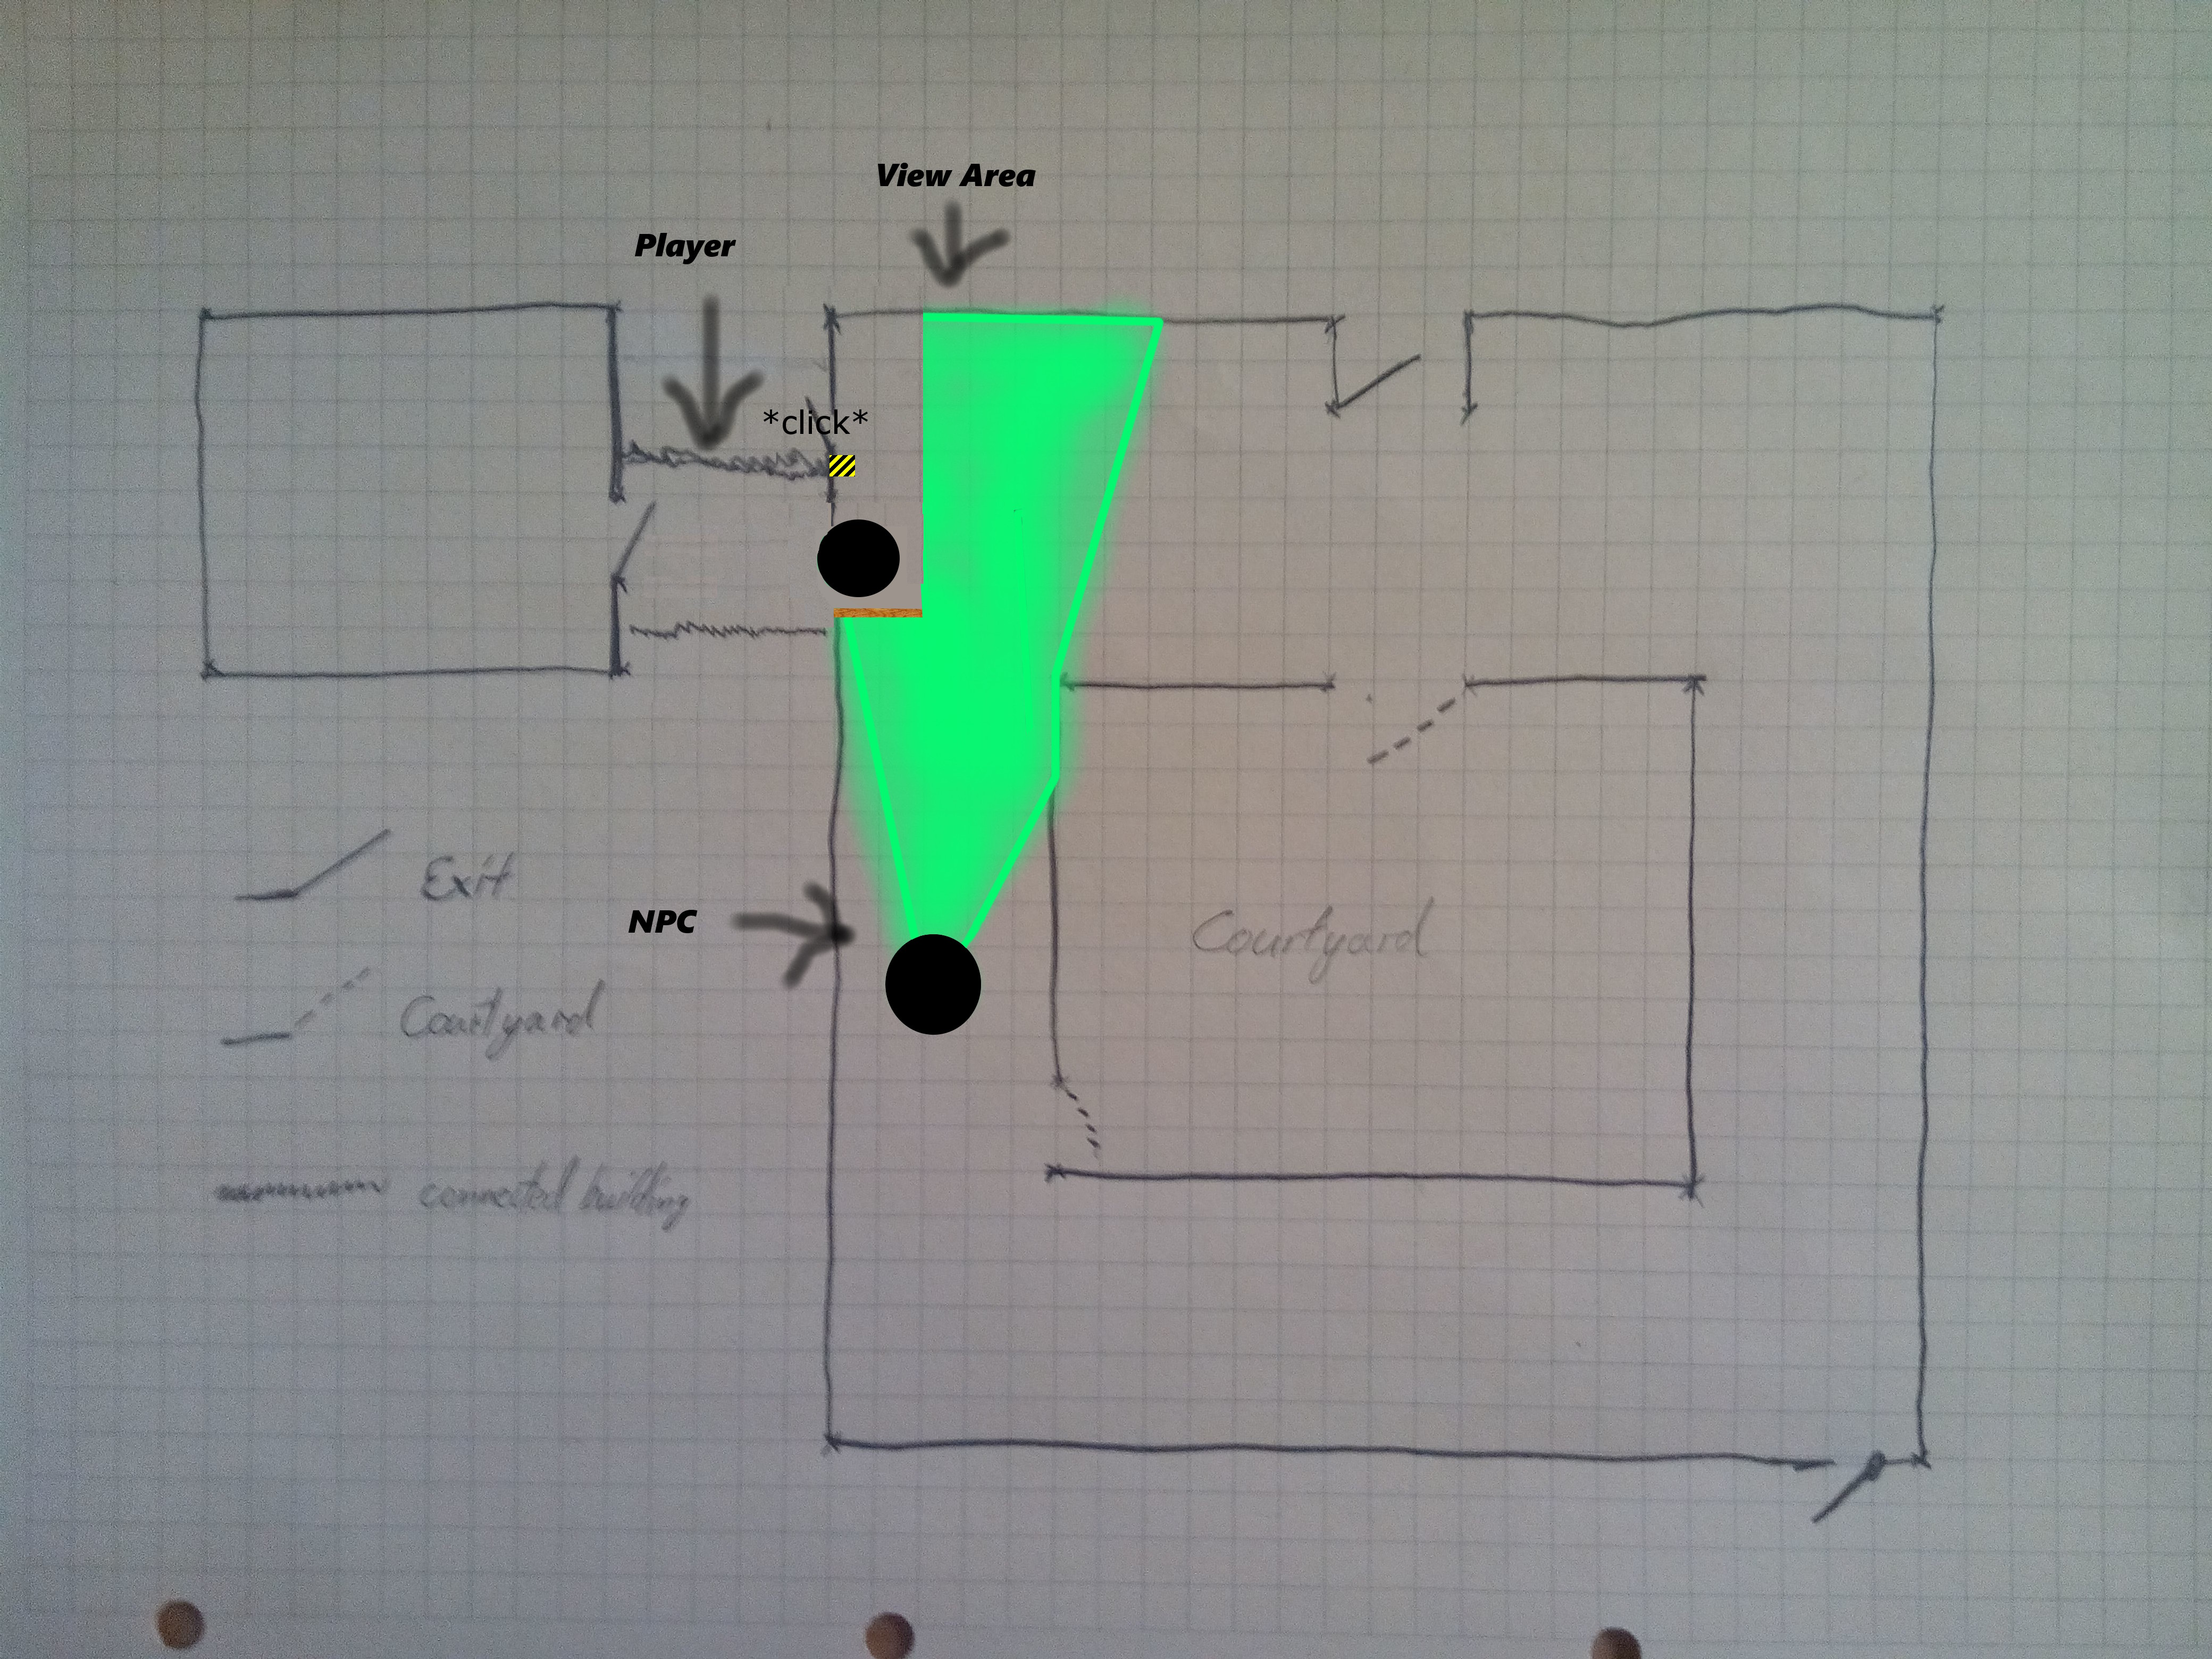
\includegraphics[width=0.9\textwidth]{Images/notgotcaught} % first figure itself
       		\caption{Use doors as a line of sight blocker to activate switches}
       	\end{minipage}\hfill
       	\begin{minipage}{0.45\textwidth}
       		\centering
       		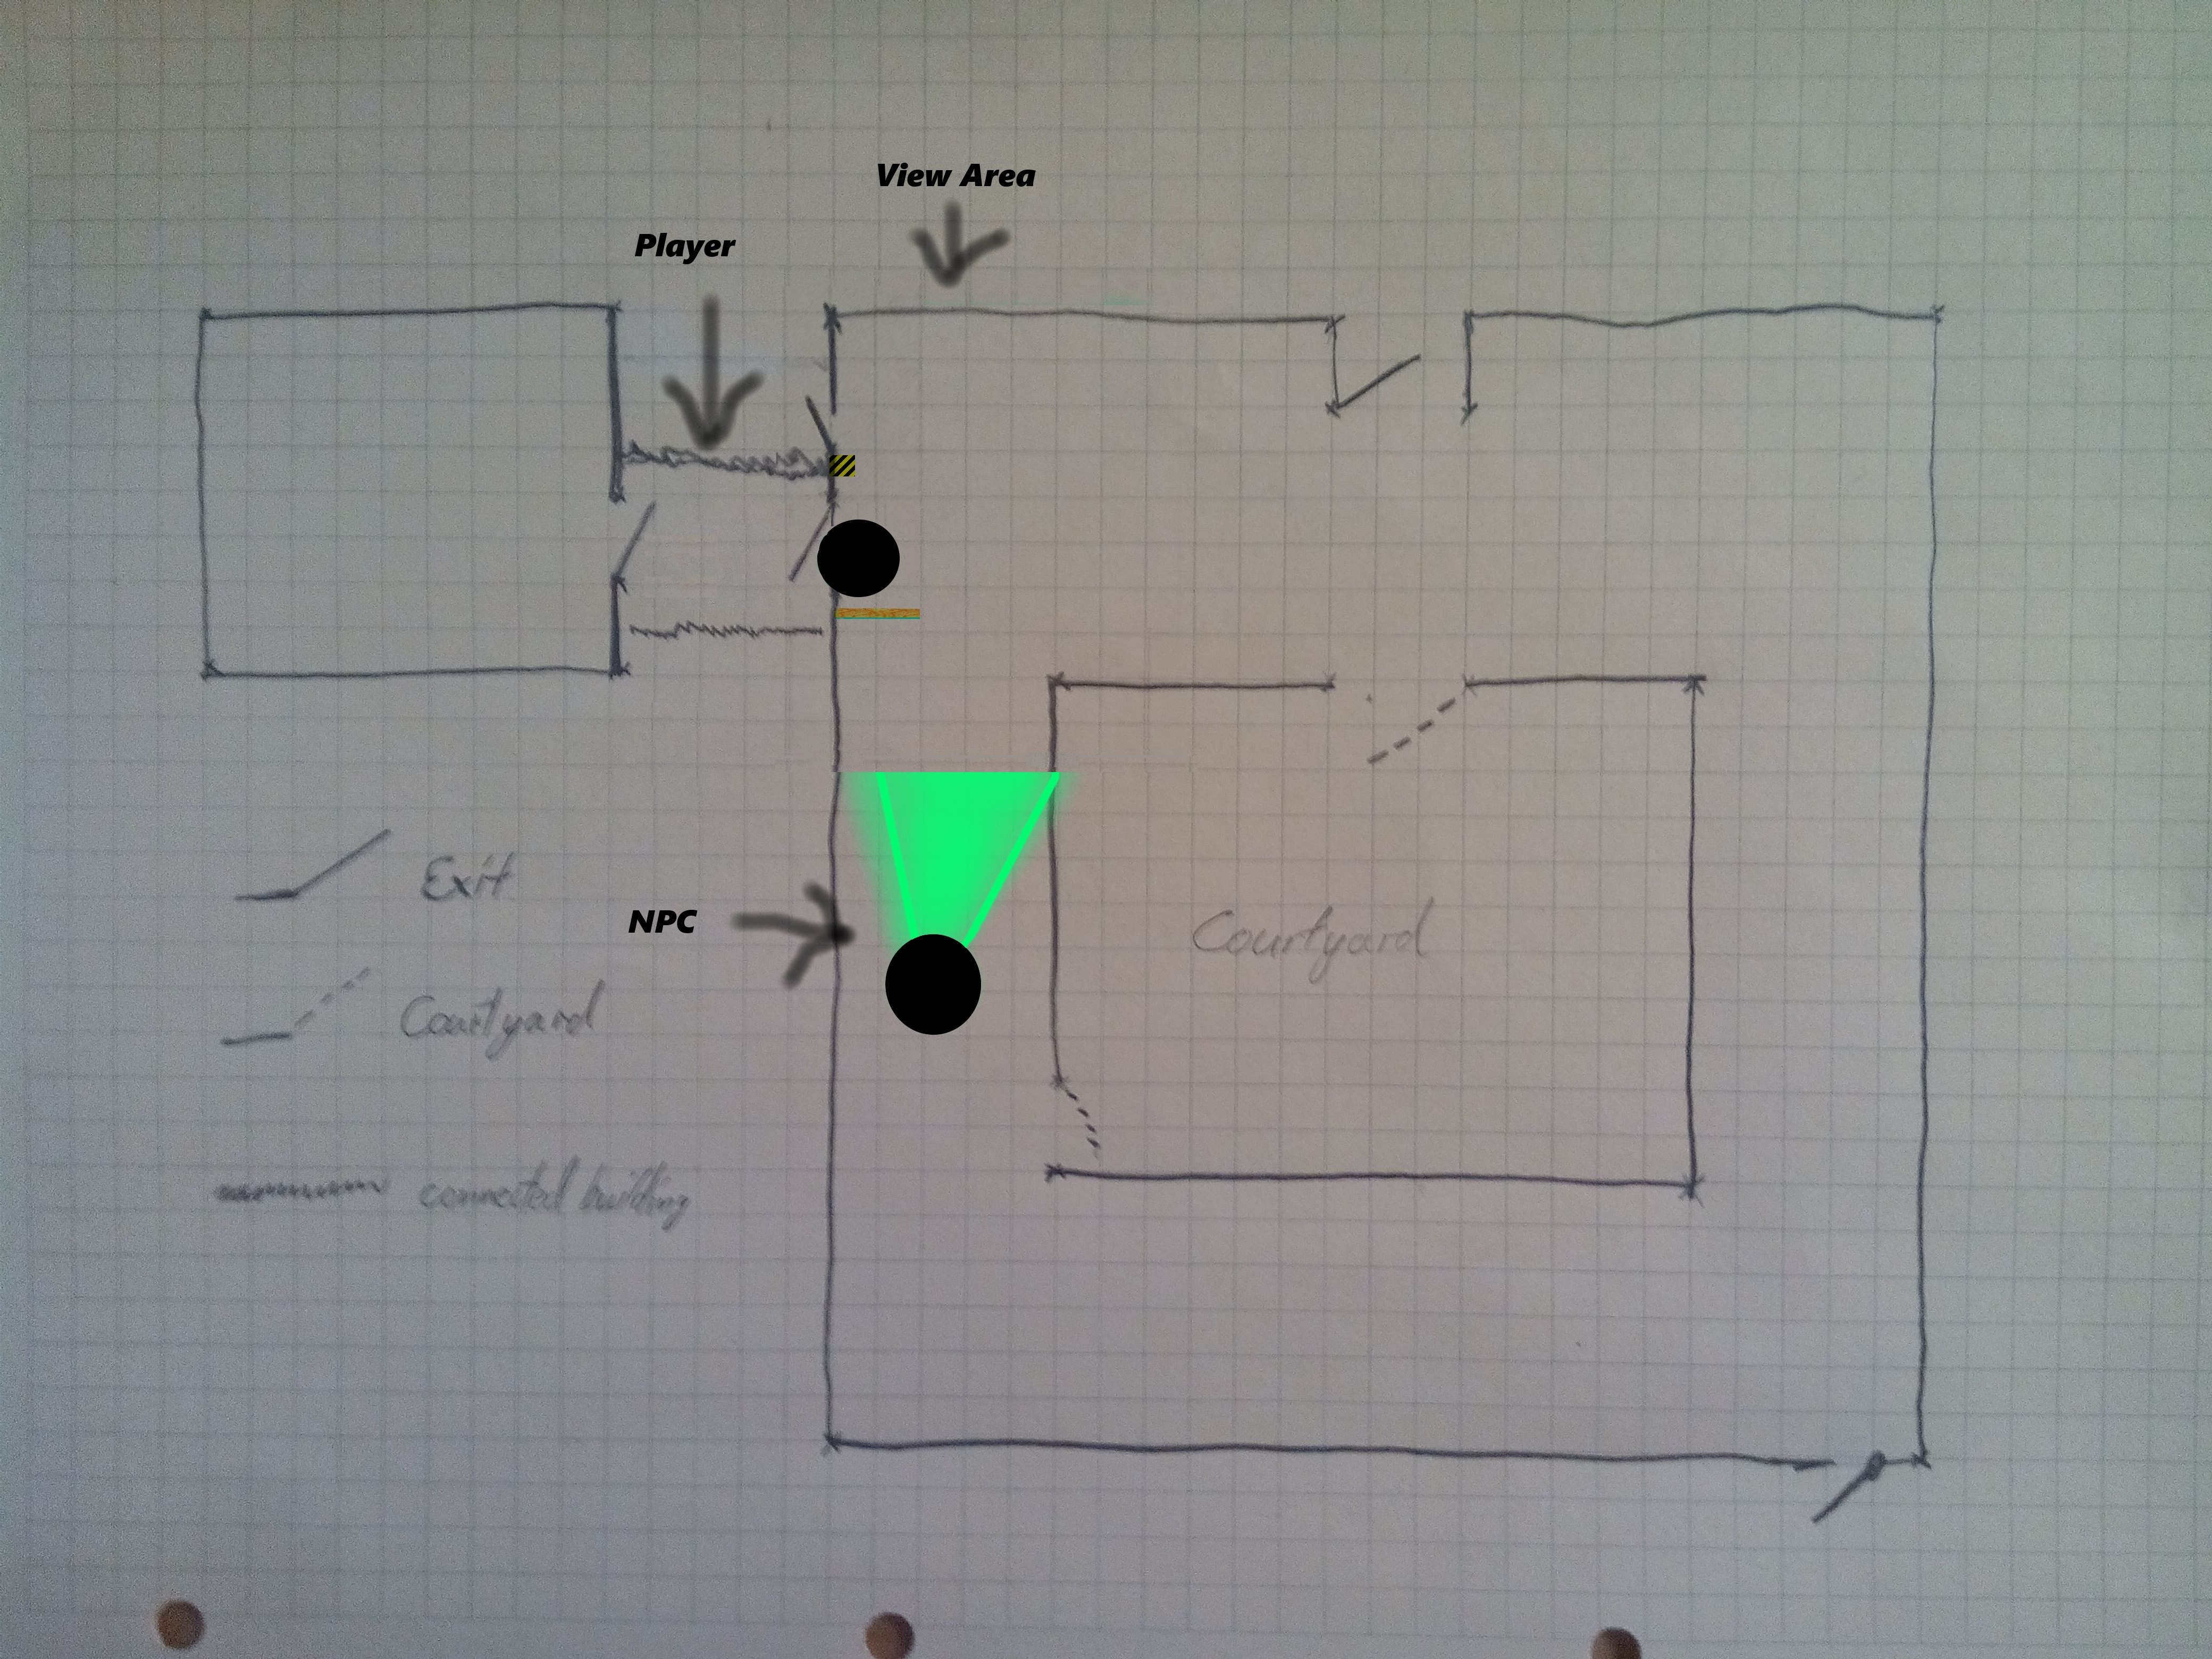
\includegraphics[width=0.9\textwidth]{Images/lightsofflineofsight} % second figure itself
       		\caption{Without light, the NPC cannot see as far as before!}
      	\end{minipage}
 \end{figure}
\end{document}
